\section{Ablation studies}
\label{sec:ablation_studies}

Alongside comparing different approaches, we also tested the effect of two design choices intended to mitigate errors on challenging images containing artifacts and cell overcrowding.

% \noindent\textbf{Artifacts Oversampling (AO)}.
\subsection{Artifacts Oversampling (AO)}

The presence of biological structures and technical artifacts like stripes, filaments (\cref{fig:artifacts:stripe}) or accidental flourophore accumulations (\cref{fig:artifacts:macaroon})  can often fool the model into detecting false positives.
% Indeed, their similarity with cells in terms of saturation and brightness makes it difficult for the model to handle them correctly. 
Indeed, their similarity with cells in terms of saturation and brightness hampers their correct handling and entices the model to overpredict.
This situation is worsened because such structures are underrepresented in the data, especially concerning the stripes and the macaroni-shaped artifact.
In fact, only a handful of artifact examples are available, which complicates their recognition even further.

For this reason, we tried to increase the augmentation factor for these inputs to facilitate the learning process.
Specifically, we selected the six different crops containing stripes and re-sampled them with the augmentation pipeline described in \cref{sec:model_training}, resulting in 150 new images for each crop.

\subsection{Weight Maps (WM)} \label{sec:weights_map}

One of the toughest challenges during the inference is related to cell overcrowding.
In particular, the cells sometimes tend to form agglomerates of several overlying neurons, making it difficult to reconstruct their individual shapes (see \cref{fig:artifacts:clumping}).
Although the human eye can often trace back the morphology of the original neurons, perhaps even piecing together missing/separated parts due to the superposition of other cells, this task is still much harder for automatic approaches.
In particular, precise object segmentation is paramount when clumps of objects are present in the images, as failing to achieve a nitid distinction of cells boundaries may lead to spurious connections between separated objects. 
If that happens, multiple objects are considered as a single one and false negatives are generated, thus deteriorating the model performance.

In order to improve cell separation, \citeA{unet} suggest leveraging a weight map that penalizes more the errors on the borders of touching cells.
Building on that, we introduce a novel implementation where single object contributions are compounded additively.
This procedure generates weights that decrease as we move away from the borders of each cell.
At the same time, the contributions coming from single items are combined so that the global weight map presents higher values where more cells are close together (see \cref{fig:weight_calculation}).
%
% \begin{figure}
% \centerline{
%      \begin{subfigure}[]{0.4\textwidth}
%          \centering
%          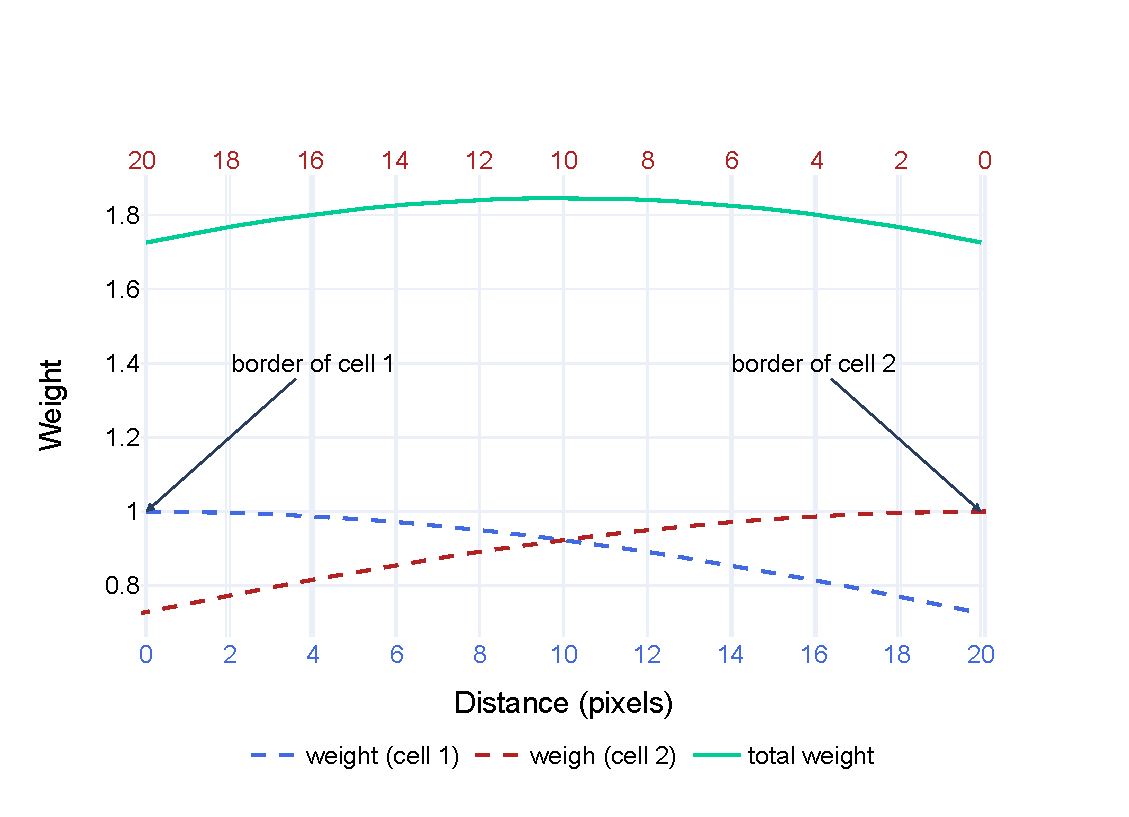
\includegraphics[width=\textwidth]{figures/130_methods/weight_calculation.eps}
%         \caption{Weight compounding}
%         \label{fig:weight_calculation}
%      \end{subfigure}
%      \begin{subfigure}[]{0.62\textwidth}
%          \centering
%          \includegraphics[ width=0.45\textwidth]{figures/130_methods/crop_mask_2451_crop.jpeg}
% \includegraphics[trim=0 0.008in 0 0, width=0.50\textwidth]{figures/130_methods/crop_weigths_2451_crop.jpeg}
%          \caption{Mask and correspondent weight map}
%          \label{fig:weight_map_example}
%      \end{subfigure}
% }
% \caption{\textbf{Weight map}. 
% \ref{fig:weight_calculation} shows the weight factors of background pixels between cells according to Eq. (\ref{weight_formula}). The dashed curves depict the weights generated by single cells as a function of the distance from their borders.
% % , respectively cell 1 on the left (blue) and cell 2 on the right (red).
% The green line illustrates the final weight obtained by adding individual contributions. 
% In \ref{fig:weight_map_example}, a target mask and the corresponding weight map.} 
% \label{fig:weight_map}
% \end{figure}
%
\begin{figure}
    \centering
    \includegraphics[width=\textwidth]{figures/130_methods/weights_calculation.pdf}
    \caption{\textbf{Weight compounding.}
    The dashed curves depict the weights generated by single cells as a function of the distance from their borders according to \cref{eq:weight_formula}.
    The green line illustrates the final weight obtained by adding individual contributions
    }
    \label{fig:weight_calculation}
\end{figure}
%
\begin{figure}
    \centering
    \subfloat[Mask]{
    \includegraphics[width=0.45\textwidth]{figures/130_methods/crop_mask_2451_crop.jpeg}
    }
    \subfloat[Weight map]{
    \includegraphics[trim=0 0.008in 0 0,
    width=0.50\textwidth]{figures/130_methods/crop_weights_2451_crop.jpeg}
    }
    \caption{\textbf{Weight map.} A target mask and the corresponding weight map}
    \label{fig:weight_map_example}
\end{figure}
%
The pseudocode\footnote{full implementation \githubweights} for a weight map is reported in Alg. \ref{algo:pseudocode_weightmap}, and an example weight map is shown in \cref{fig:weight_map_example}.

\begin{algorithm}%[H]
% \begin{algorithmic}[1]
\DontPrintSemicolon
     Initialize empty $\text{map}_j$ (mask size)\tcp*{weight map $j$-th mask}
    \For{each cell in mask} 
    {
    \tcc{loop over $i$-th cell in $j$-th mask}
         Initialize empty $\text{map}_i$  (mask size) \tcp*{weight map $i$-th cell}
        
         Add $i$-th cell to $\text{map}_i$
        
         Compute euclidean distance between each pixel of $\text{map}_i$ and the closest pixel of the $i$-th cell \label{step:distance}
        
         Compute each pixel's weight in $\text{map}_i$ according to a decreasing exponential function:
        \begin{equation}
        % \hskip 4.5cm
        \text{weight} = \exp\left\{\dfrac{-d^{2}}{2\sigma^{2}}\right\}
        \label{eq:weight_formula}
        \end{equation}
        
        \tcc {$d$ is the distance computed at step \ref{step:distance}}
        \tcc {$\sigma$ is a customizable parameter set to 25 (average cell radius)}
        
    Sum the resulting $\text{map}_i$ to the full $\text{map}_j$
    % , as illustrated in Fig. \ref{fig:weight_calculation};
}
% \end{algorithmic}
\caption{weight map pseudocode for $j$-th mask}
\label{algo:pseudocode_weightmap}
\end{algorithm}
